\documentclass{beamer}
\usepackage{blindtext}
\usepackage{graphicx}
\usepackage[spanish]{babel}
\usepackage[utf8]{inputenc}
\usetheme{Madrid}

\title{Object-Z}

\author{Christofer Chávez Carazas \and Juan León Camilo}

\institute[Universidad Nacional de San Agustin] % (optional, but mostly needed)
{
  Universidad Nacional de San Agustín
}

\date{\today}



\begin{document}

\maketitle

\begin{frame}{Introducción}
    \begin{itemize}
        \item Object-Z es una extensión orientada a objetos del lenguaje de especificación Z. 
        \item Object-Z añade a Z formas de expresar conceptos del paradigma orientado a objetos, sobre todo clases, polimorfismo y herencia.
    \end{itemize}
\end{frame}

\begin{frame}{Ejemplo de las Tarjetas de crédito}
  \begin{itemize}
      \item El sistema está previsto de una colección de cuentas de tarjetas de crédito.
      \item Cada cuenta tiene dos números, el balance actual y el crédito límite.
      \item El dinero puede ser retirado o depositado.
  \end{itemize}
\end{frame}

\begin{frame}{Class}
    \begin{figure}
        \centering
        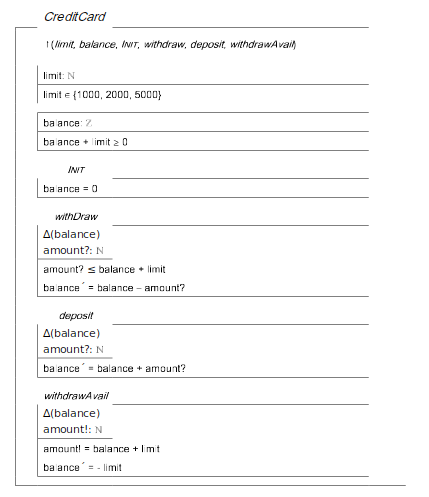
\includegraphics[scale=0.3]{Z1.png}
        \caption{Class}
        \label{Clase CreditCard}
    \end{figure}
\end{frame}

\begin{frame}{Visibility list}
  \begin{figure}
      \centering
      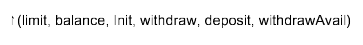
\includegraphics[scale=0.5]{Z2.png}
      \caption{Visibility list}
      \label{Visibility List}
  \end{figure}
  \begin{itemize}
      \item Son as partes y componenetes que son visibles en el entorno de un objeto Tarjeta de Crédito.
      \item Si la visibility list es omitida, se deducirá que todos los componentes de la clase son visibles.
  \end{itemize}
\end{frame}

\begin{frame}{Definición de constantes}
  \begin{figure}
      \centering
      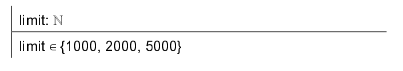
\includegraphics[scale=0.5]{Z3.png}
      \caption{Constantes}
      \label{Constantes}
  \end{figure}
  \begin{itemize}
   \item Se grafica con una caja abierta.
   \item La parte de arriba es una tipica declaración en Z de una lista.
   \item Y la parte de abajo los valores de la lista.
  \end{itemize}
\end{frame}

\begin{frame}{Esquema de estado}
  \begin{figure}
      \centering
      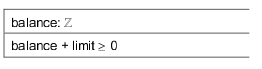
\includegraphics[scale=0.5]{Z4.png}
      \caption{State Schema}
      \label{Esquema de estado}
  \end{figure}
  \begin{itemize}
   \item Se grafica con una caja cerrada sin nombre.
   \item Se utiliza el mismo patrón que en la definición de las constantes.
   \item Aquí se definen las variables.
  \end{itemize}
\end{frame}

\begin{frame}{Esquema Inicial}
  \begin{figure}
      \centering
      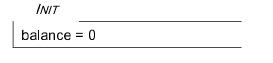
\includegraphics[scale=0.5]{Z5.png}
      \caption{Initial Schema }
      \label{Esquema Inicial}
  \end{figure}
  \begin{itemize}
   \item Se grafica con una caja cerrada nombrada con la palabra INIT.
   \item Se inicializan las variables.
   \item El predicado inicial debe ser verdadero para todas las variables.
  \end{itemize}
\end{frame}

\begin{frame}{Esquemas de }
  \begin{figure}
      \centering
      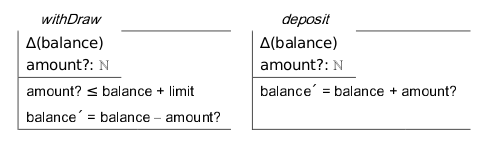
\includegraphics[scale=0.5]{Z6.png}
      \caption{Operation Schema}
      \label{Esquema de operacion}
  \end{figure}
 \begin{itemize}
  \item Los esquemas se definen de la misma forma que el lenguaje Z.
 \end{itemize}
\end{frame}

\begin{frame}{TwoCards}
  \begin{figure}
      \centering
      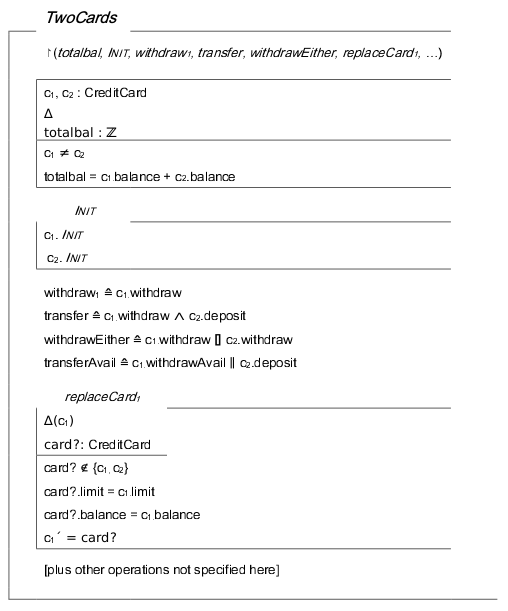
\includegraphics[scale=0.3]{Z7.png}
      \caption{TwoCards}
      \label{Clase TwoCards}
  \end{figure}
\end{frame}

\begin{frame}{Variables secundarias}
  \begin{figure}
      \centering
      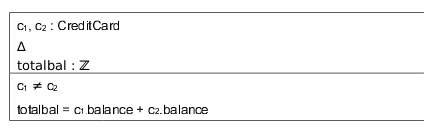
\includegraphics[scale=0.5]{Z8.png}
      \caption{Secondary Variables}
      \label{Variables secundarias}
  \end{figure}
  \begin{figure}
  \item Las variables secundarias son declaradas en terminos de las variables primarias.
  \end{figure}
\end{frame}

\begin{frame}{Esquma inicial}
  \begin{figure}
      \centering
      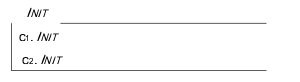
\includegraphics[scale=0.5]{Z9.png}
      \caption{Inital Schema}
      \label{Esquema Inicial}
  \end{figure}
\end{frame}

\begin{frame}{Expresiones de operación}
 \begin{figure}
      \centering
      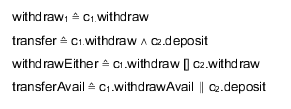
\includegraphics[scale=0.5]{Z10.png}
      \caption{Operation expressions}
      \label{Esquema Inicial}
  \end{figure}
  \begin{itemize}
   \item \textbf{Expresion de Conjunción: } Símbolo: $\wedge$
   \item \textbf{Expresion de Elección:} Símbolo: $\Box$
   \item \textbf{Composición Paralela:} Símbolo: $\parallel$
   \item \textbf{Composición Secuencial:} Símbolo: ;
  \end{itemize}
\end{frame}

\begin{frame}{CreditCards}
  \begin{figure}
      \centering
      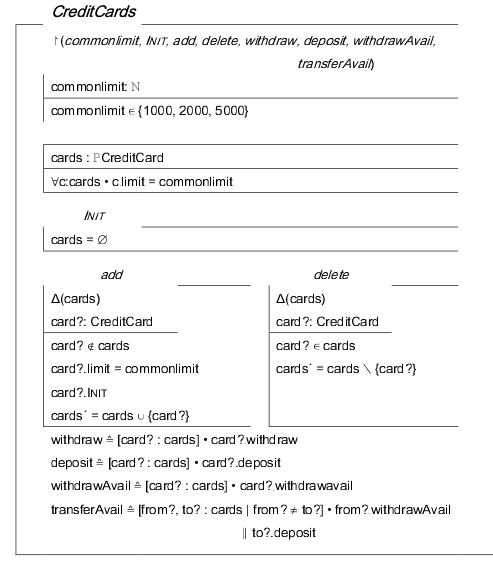
\includegraphics[scale=0.3]{Z11.png}
      \caption{CreditCards}
      \label{Tarjetas de Credito}
  \end{figure}
\end{frame}


\begin{frame}{Herencia}
 \begin{figure}
      \centering
      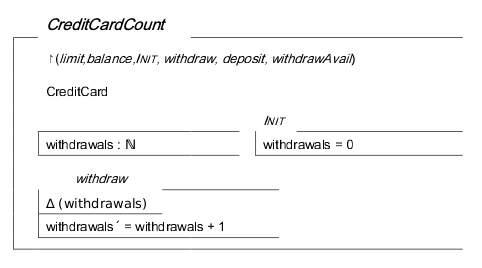
\includegraphics[scale=0.5]{Z12.png}
      \caption{CreditCards}
      \label{Tarjetas de Credito}
  \end{figure}
\end{frame}

\begin{frame}{Bibliografía}
  \begin{thebibliography}{10}
  \beamertemplatebookbibitems
  \bibitem{Author1990}
    Tim G. Kimber
    \newblock {\em Object-Z to Perfect Developer}
    \newblock {Chapter 2. Object-Z}
    \newblock {Imperial College London, 2007}
  \end{thebibliography}
\end{frame}

\end{document}


